Relacionado a los resultados del algoritmo 1. Este algoritmo tardó un total de $3$ generaciones en alcanzar el criterio de paro por épsilon, obteniendo una aptitud promedio final de $0.9583$ y presentando a su mejor individuo con aptitud de $1.0000$. El proceso de convergencia se puede observar en la Figura \ref{fig: m_op}.

\begin{figure}[htbp]
	\centering
	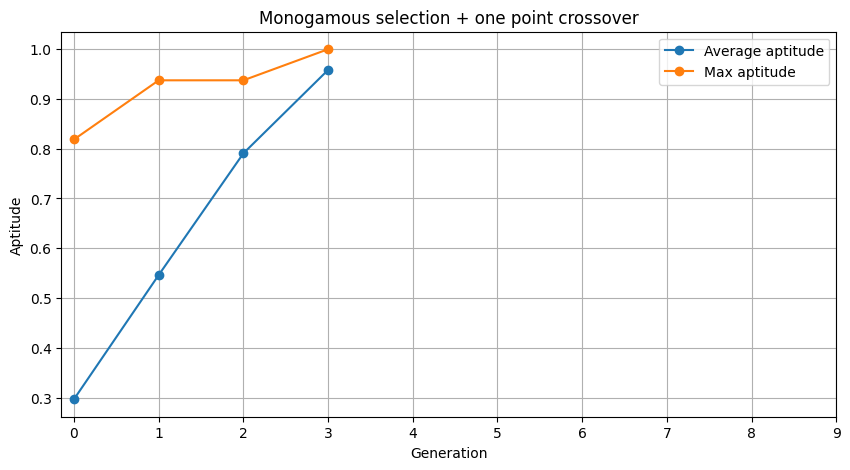
\includegraphics[width=0.4\textwidth]{monogamous_selection_one_point_crossover}
	\caption{Evolución de la aptitud de los individuos del algoritmo 1.}
	\label{fig: m_op}
\end{figure}

Este algoritmo muestra un buen rendimiento en términos de aptitud promedio y mejor aptitud, ya que logra una aptitud promedio alta y alcanza la mejor aptitud posible de $1$. Sin embargo, se requirieron 3 generaciones para llegar a este punto. Es posible que el algoritmo haya tenido que explorar varias soluciones antes de converger a la solución óptima.

Respecto al desempeño del algoritmo 2. Se tomó un total de $2$ generaciones en alcanzar el criterio de paro por épsilon, presentando una aptitud promedio final de $0.8434$ y teniendo a su mejor individuo con aptitud de $1.0000$. Este proceso de evolución se puede observar en la Figura \ref{fig: m_tp}.

\begin{figure}[htbp]
	\centering
	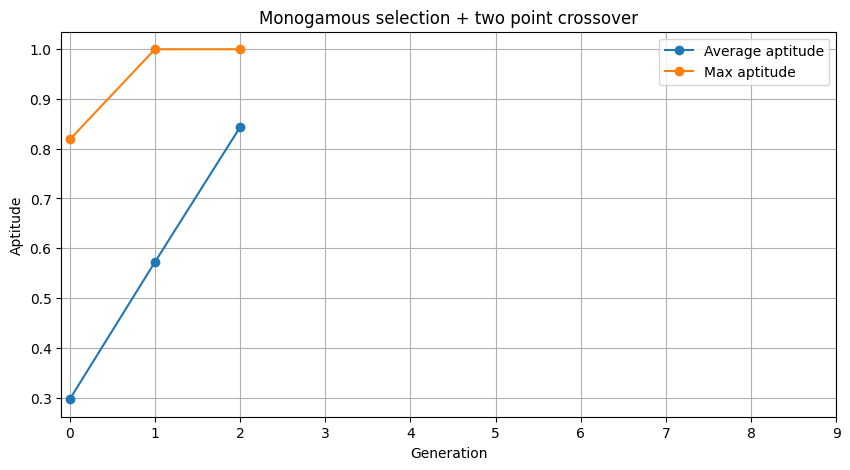
\includegraphics[width=0.4\textwidth]{monogamous_selection_two_point_crossover}
	\caption{Evolución de la aptitud de los individuos del algoritmo 2.}
	\label{fig: m_tp}
\end{figure}

En este caso, también presenta una alta mejor aptitud de $1$, pero en comparación con el Algoritmo 1, requiere solo $2$ generaciones. Aunque el valor promedio de aptitud es menor que el del Algoritmo 1, la rápida convergencia en solo $2$ generaciones es una característica destacable.

En cuanto al algoritmo 3. Este tardó un total de $5$ generaciones en alcanzar el paro por épsilon, logrando obtener una aptitud promedio final de $0.8219$, y teniendo a su mejor individuo con una aptitud de $1.0000$. Para este algoritmo podemos observar en la Figura \ref{fig: p_op} su proceso de evolución.

\begin{figure}[htbp]
	\centering
	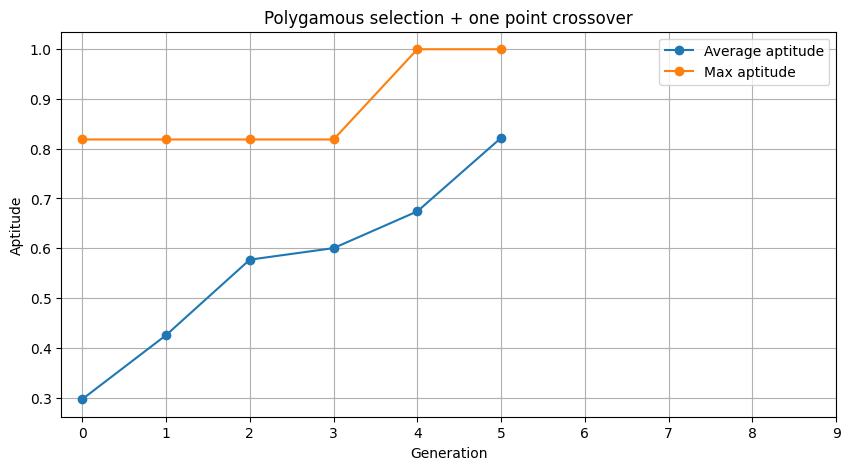
\includegraphics[width=0.4\textwidth]{polygamous_selection_one_point_crossover}
	\caption{Evolución de la aptitud de los individuos del algoritmo 3.}
	\label{fig: p_op}
\end{figure}

Dicho algoritmo tiene un mayor número de generaciones en comparación con los dos algoritmos anteriores. Aunque la aptitud promedio y la mejor aptitud siguen siendo altas, el mayor número de generaciones podría indicar que este algoritmo requiere más tiempo para converger hacia soluciones óptimas.

Por último, relacionado al algoritmo 4. Se tomo un total de $2$ generaciones en alcanzar el paro por épsilon, donde se obtuvo una aptitud promedio final de $0.8185$, y un mejor individuo con un valor igual de aptitud. El proceso de evolución de este algoritmo se puede observa en la Figura \ref{fig: p_tp}.

\begin{figure}[htbp]
	\centering
	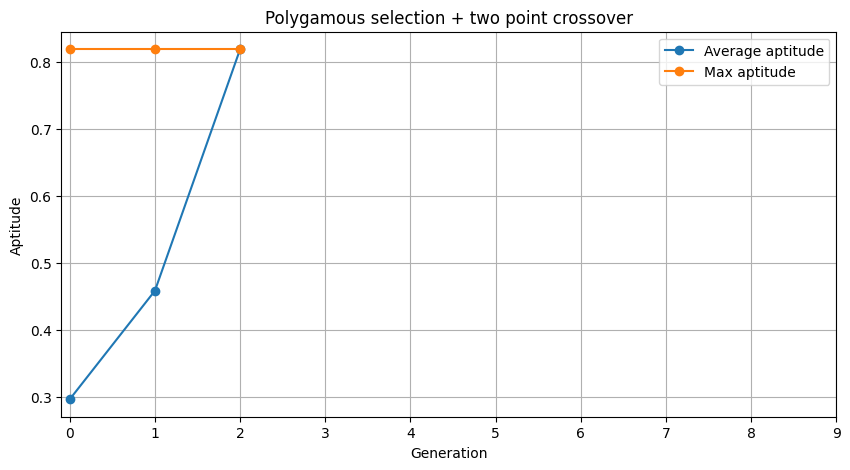
\includegraphics[width=0.4\textwidth]{polygamous_selection_two_point_crossover}
	\caption{Evolución de la aptitud de los individuos del algoritmo 4.}
	\label{fig: p_tp}
\end{figure}

Es importante notar que la mejor aptitud de este algoritmo no alcanza el valor máximo posible de $1$. Aunque este algoritmo requiere solo $2$ generaciones, su incapacidad para alcanzar la mejor aptitud posible podría indicar que está quedando atrapado en un óptimo local o necesita ajustes en su configuración.